% Created 2018-11-25 Sun 05:12
% Intended LaTeX compiler: lualatex
\documentclass[10pt, presentation, colorlinks]{beamer}
\usepackage{graphicx}
\usepackage{grffile}
\usepackage{longtable}
\usepackage{wrapfig}
\usepackage{rotating}
\usepackage[normalem]{ulem}
\usepackage{amsmath}
\usepackage{textcomp}
\usepackage{amssymb}
\usepackage{capt-of}
\usepackage{hyperref}
% settings for code hightliting
\definecolor{back}{RGB}{250,250,250}  % should match to bg color
\definecolor{keywords}{RGB}{255,0,90}
\definecolor{comments}{RGB}{60,179,113}
\usepackage{listings} % code hightliting package (required `fragile` for frame )
\lstset{language=Scala, columns=fixed,basicstyle=\normalsize\ttfamily, morekeywords={Option, ClassTag}, keywordstyle=\color{keywords}, backgroundcolor=\color{back}, keepspaces=true, stringstyle=\color{comments}, commentstyle=\color{comments}\emph}
% colors and commands for tables
\definecolor{coolGreen}{HTML}{096c31}
\newcommand{\clm}[1]{\textcolor{coolGreen}{\rotatebox{90}{\textbf{\large #1}}}}
\newcommand{\row}[1]{\textbf{\large #1}}
\usetheme[titleformat=smallcaps, sectionpage=simple,numbering=counter, progressbar=frametitle]{metropolis}
\author{Evgeniy T}
\date{2018}
\title{How To Write Nice Looking Presentation With Beamer And Org-Mode}
% metropolis fonts set up
\setsansfont[ItalicFont={Fira Sans Italic},BoldItalicFont={Fira Sans Bold Italic}, BoldFont={Fira Sans Bold}]{Fira Sans Regular}
\setmonofont{Iosevka SS08 Semibold}
% Use notes with PDFPC or with Dspdfviewer
\usepackage{pgfpages}
\setbeameroption{show notes on second screen=right}
% As workaround for notes on second screen with Metropolis theme (bug at Beamer) use Lualatex
% customize links color
\definecolor{links}{HTML}{0061A4}
\hypersetup{colorlinks,linkcolor=,urlcolor=links}
\hypersetup{
 pdfauthor={Evgeniy T},
 pdftitle={How To Write Nice Looking Presentation With Beamer And Org-Mode},
 pdfkeywords={},
 pdfsubject={},
 pdfcreator={Emacs 27.0.50 (Org mode 9.1.9)},
 pdflang={English}}
\begin{document}

\maketitle

\begin{frame}[label={sec:org037e95c}]{Links}
\begin{block}{tutorial: \url{https://orgmode.org/worg/exporters/beamer/tutorial.html}}
\end{block}

\begin{block}{beamer export: \url{https://orgmode.org/manual/Beamer-export.html}}
\end{block}

\begin{block}{latex export: \url{https://orgmode.org/manual/LaTeX-export.html\#LaTeX-export}}
\end{block}

\begin{block}{Theme \url{https://github.com/matze/mtheme}  or  \url{https://github.com/rchurchley/beamercolortheme-owl}}
\end{block}

\begin{block}{Cheat Sheet  \url{https://github.com/fniessen/refcard-org-beamer}}
\end{block}

\note{Note
Use it for store speaker notes with advanced PDF viewers such as PDFPC \url{https://pdfpc.github.io/}
(see: \url{https://tex.stackexchange.com/questions/84622/is-there-a-specialized-pdf-viewer-for-latex-beamer-presentations-on-linux})}
\end{frame}


\begin{frame}[fragile,label={sec:org1349e61}]{Code Block Without Highlighting}
 Just text.

\begin{verbatim}
val test = 1 + 5
println(test.toString)
\end{verbatim}

\note{Note
Just note example}
\end{frame}

\begin{frame}[fragile,label={sec:org0794629}]{Code Block With Highlighting}
\begin{block}{use latex export block with the "lstlisting" package:}
\begin{itemize}
\item Tutorial: \url{https://mikedewar.wordpress.com/2009/02/25/latex-beamer-python-beauty/}
\item docs: \url{https://en.wikibooks.org/wiki/LaTeX/Source\_Code\_Listings}
\end{itemize}


\begin{lstlisting}
// simple code example
def parseOpt[A: ClassTag](a: Any): Option[A] =
  a match {
    case a: A => Some(a)
    case _ => None
  }
}

def xxx[A](a: Int) = "000"
\end{lstlisting}
\end{block}
\end{frame}

\begin{frame}[label=, standout]{Standout}
\begin{itemize}
\item pure \alert{FP}
\item composition
\item streaming
\end{itemize}
\end{frame}

\begin{frame}[label={sec:org6a2883d}]{Table}
\def\arraystretch{1.4} % height of the row
\begin{center}
\large
\begin{tabular}{|c|c|c|c|}
\hline
\clm{a} & \clm{name} & \clm{long name} & \clm{other}\\
\hline
\row{b} & V & 0 & Lorem ipsum met\\
\hline
\row{c} & 0 & Excepteur cupidatat & Ut minim, quis  exercitation\\
 &  &  & \\
\hline
\end{tabular}
\end{center}
\end{frame}


\begin{frame}[fragile,label={sec:orgfd17270}]{Columns Blocks}
 \emph{\uline{\alert{Just Text}}}

\begin{columns}
\begin{column}{0.45\columnwidth}
\begin{block}{}
\begin{verbatim}
sealed trait MarkStyle
case class PointStyle(
  color: Color,
  borderColor: Color,
  bolderWidth: Double,
  radius: Double,
  shape: PointShape
) extends MarkStyle
\end{verbatim}
\end{block}
\end{column}

\begin{column}{0.45\columnwidth}
\begin{block}{}
\begin{verbatim}
case class FontStyle(
   name: String,
   weight: FontWeight,
   size: Double,
   color: Color
 ) extends MarkStyle
\end{verbatim}
\end{block}
\end{column}
\end{columns}
\end{frame}


\begin{frame}[label={sec:org71fa437}]{Image}
\begin{center}
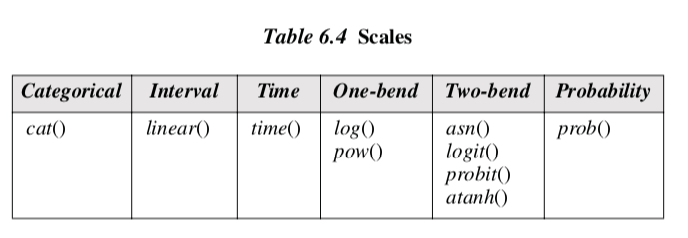
\includegraphics[height=3cm]{./img/algebra-scales.png}
\end{center}
\end{frame}

\begin{frame}[label={sec:org1f6e513}]{Ditaa}
\begin{center}
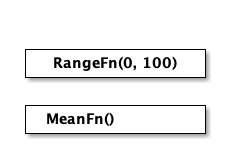
\includegraphics[width=7cm]{./img/ditaa-sample.png}
\end{center}
\end{frame}
\end{document}
